\documentclass[11pt]{article}
\usepackage{amssymb,amsfonts,amsmath,amsthm}
\usepackage[polish]{babel}
\usepackage[utf8]{inputenc}
\usepackage[T1]{fontenc}
\usepackage{graphicx}






\title{Sprawozdanie Algorytmy}
\begin{document}
	\maketitle
	
	\pagestyle{empty}
	
\begin{figure}
	\section{Wykresy zależności czasu od liczby elementów według algorytmu.}
	\centering
	
	\begin{minipage}{0.48\textwidth}
		\hspace*{-5cm}
		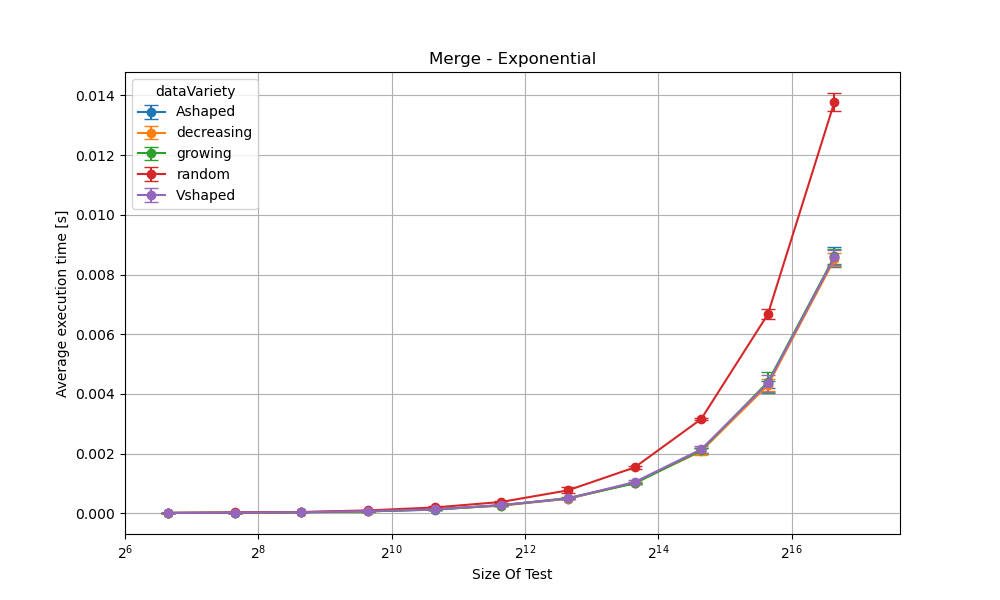
\includegraphics[scale=0.7]{../plotsAlgo/Merge_Exponential.png}
		\caption{Merge – Exponential}
		\label{fig:merge_exponential}
	\end{minipage}
	\hfill
	
	\begin{minipage}{0.48\textwidth}
		\hspace*{-5cm}
		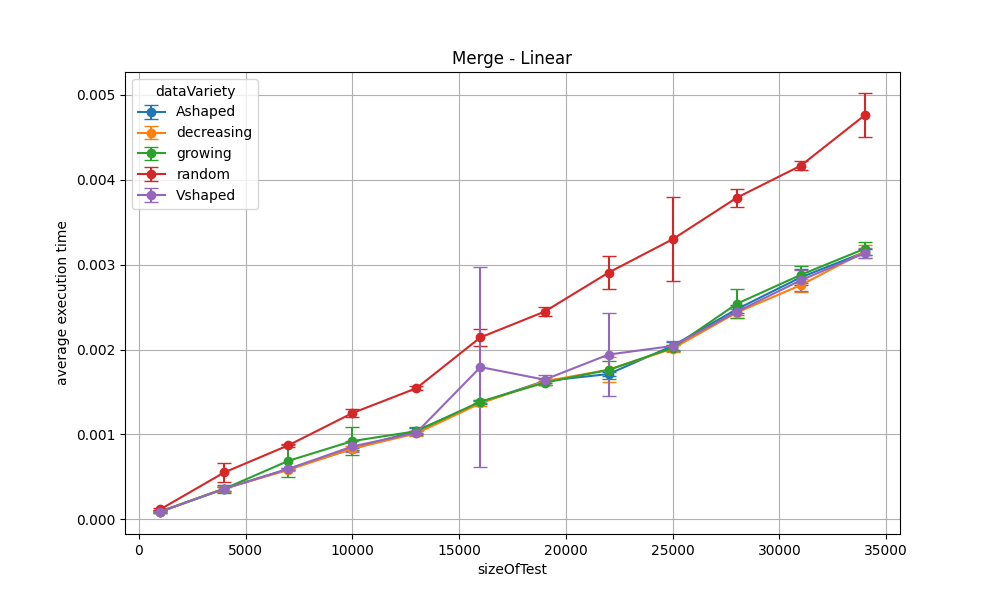
\includegraphics[scale=0.7]{../plotsAlgo/Merge_Linear.png}
		\caption{Merge – Linear}
		\label{fig:merge_linear}
	\end{minipage}
	
\end{figure}

\begin{figure}
	\centering
	
	\begin{minipage}{0.48\textwidth}
		\hspace*{-5cm}
		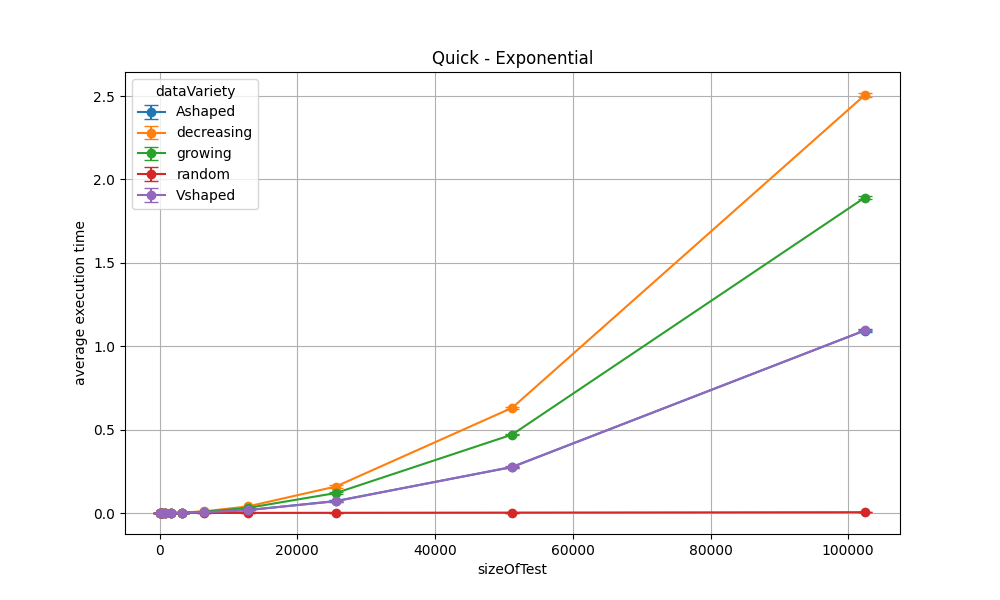
\includegraphics[scale=0.7]{../plotsAlgo/Quick_Exponential.png}
		\caption{Quick – Exponential}
		\label{fig:quick_exponential}
	\end{minipage}
	\hfill
	
	\begin{minipage}{0.48\textwidth}
		\hspace*{-5cm}
		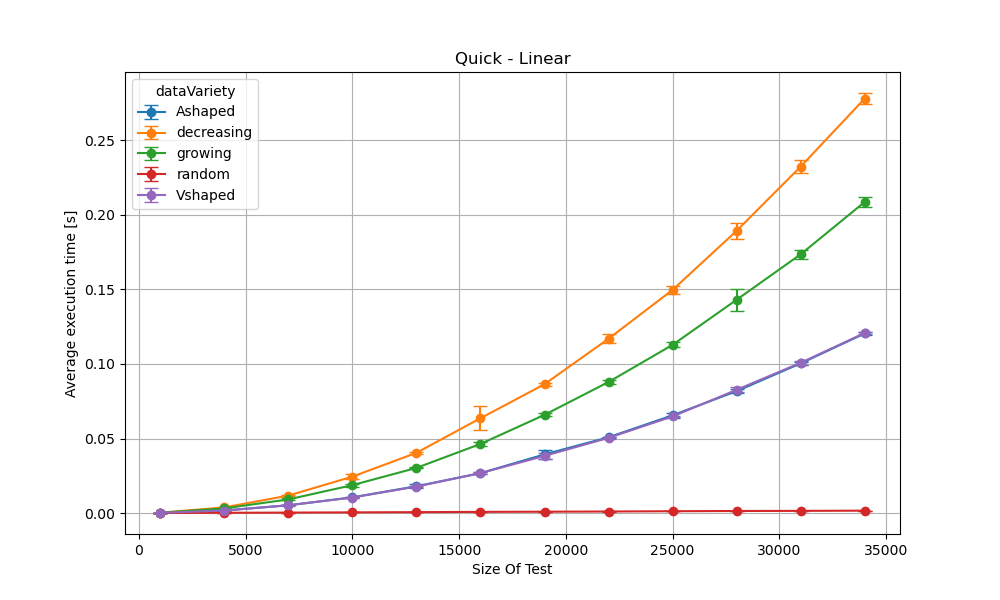
\includegraphics[scale=0.7]{../plotsAlgo/Quick_Linear.png}
		\caption{Quick – Linear}
		\label{fig:quick_linear}
	\end{minipage}
	
\end{figure}

\begin{figure}
	\centering
	
	\begin{minipage}{0.48\textwidth}
		\hspace*{-5cm}
		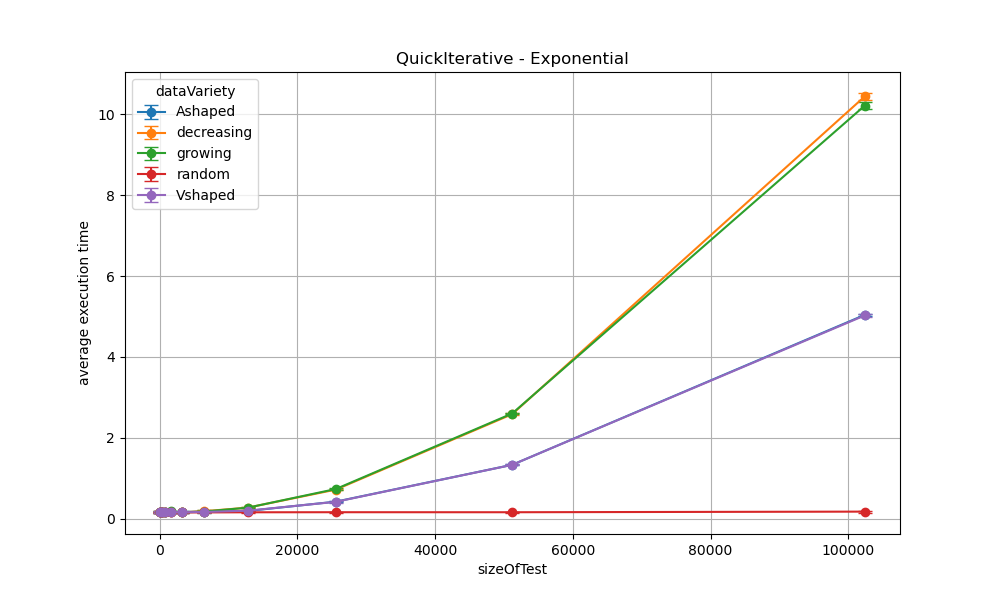
\includegraphics[scale=0.7]{../plotsAlgo/QuickIterative_Exponential.png}
		\caption{QuickIterative – Exponential}
		\label{fig:quickiterative_exponential}
	\end{minipage}
	\hfill
	
	\begin{minipage}{0.48\textwidth}
		\hspace*{-5cm}
		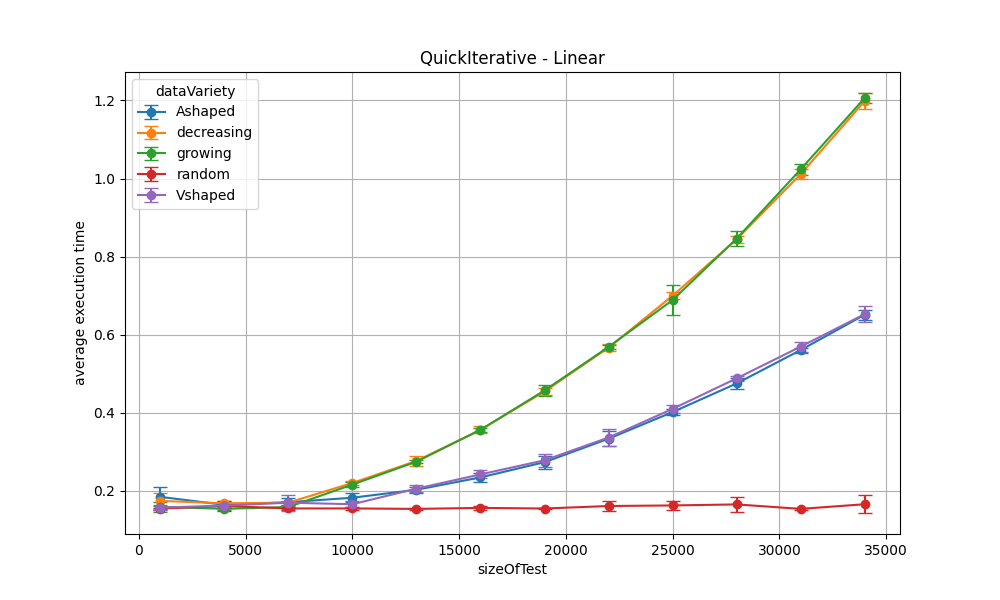
\includegraphics[scale=0.7]{../plotsAlgo/QuickIterative_Linear.png}
		\caption{QuickIterative – Linear}
		\label{fig:quickiterative_linear}
	\end{minipage}
	
\end{figure}

\begin{figure}
	\centering
	
	\begin{minipage}{0.48\textwidth}
		\hspace*{-5cm}
		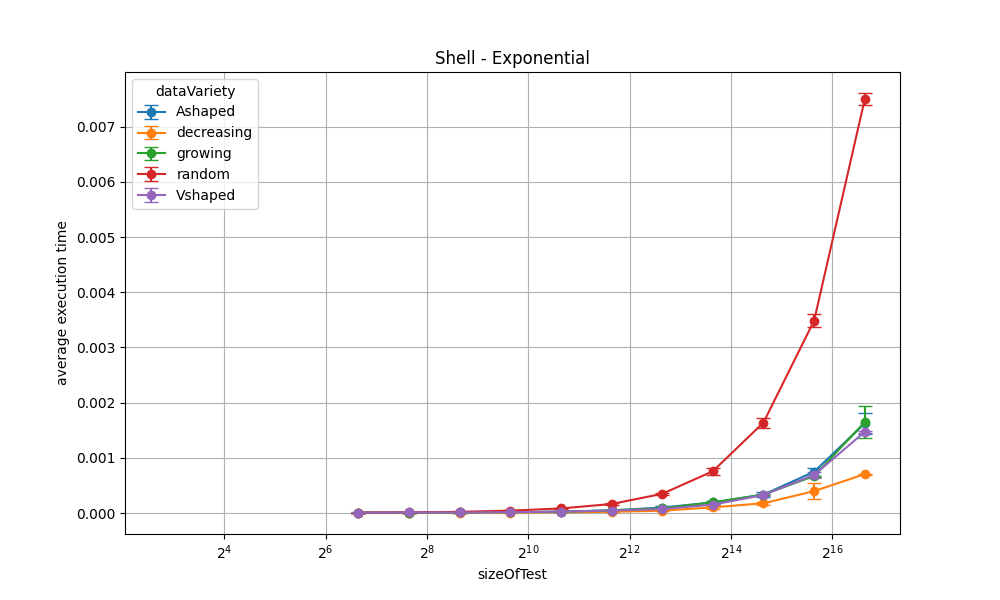
\includegraphics[scale=0.7]{../plotsAlgo/Shell_Exponential.png}
		\caption{Shell – Exponential}
		\label{fig:shell_exponential}
	\end{minipage}
	\hfill
	
	\begin{minipage}{0.48\textwidth}
		\hspace*{-5cm}
		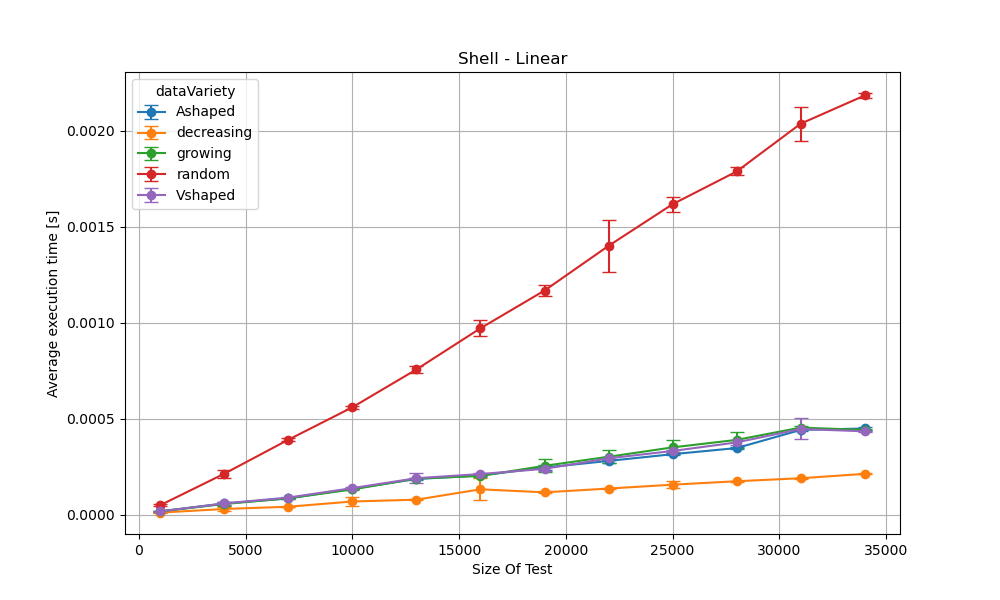
\includegraphics[scale=0.7]{../plotsAlgo/Shell_Linear.png}
		\caption{Shell – Linear}
		\label{fig:shell_linear}
	\end{minipage}
	
\end{figure}
\clearpage




\begin{figure}
	\section{Wykresy zależności czasu od liczby elementów według algorytmu.}
	\centering
	
	\begin{minipage}{0.48\textwidth}
		\hspace*{-5cm}
		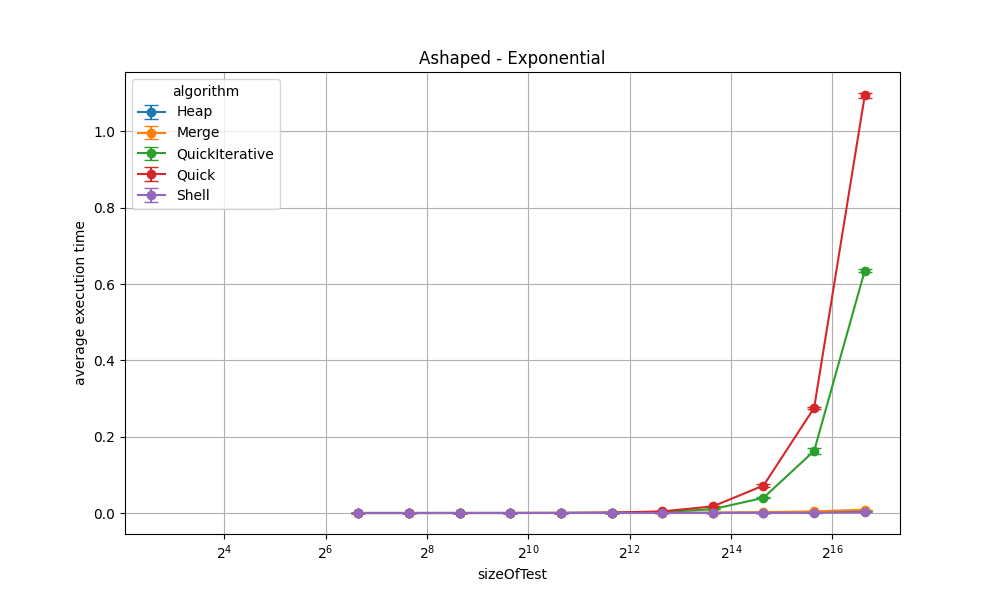
\includegraphics[scale=0.7]{../plotsData/Ashaped_Exponential.png}
		\caption{A-shaped – Exponential}
		\label{fig:ashaped_exponential}
	\end{minipage}
	\hfill
	
	\begin{minipage}{0.48\textwidth}
		\hspace*{-5cm}
		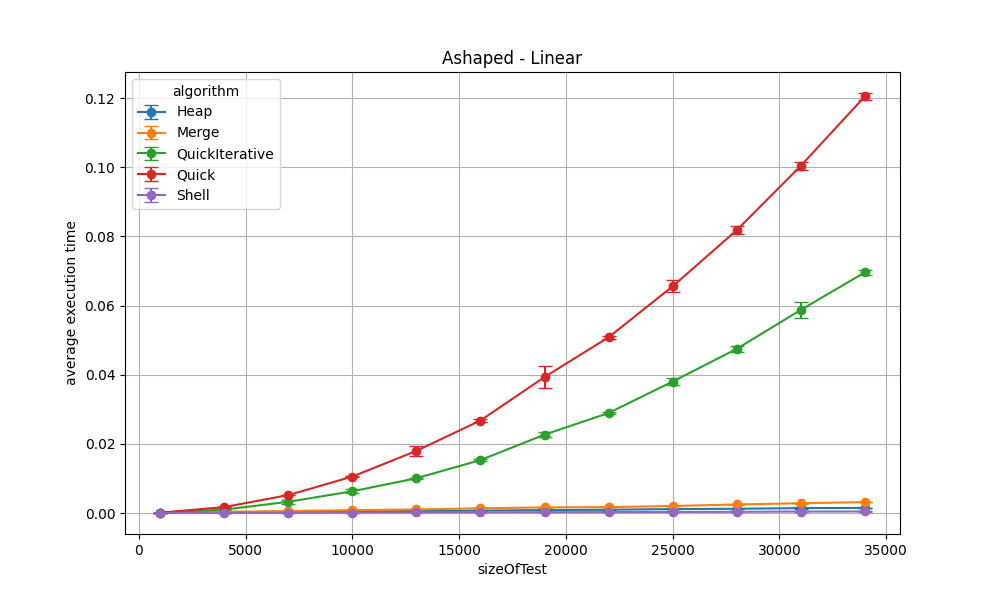
\includegraphics[scale=0.7]{../plotsData/Ashaped_Linear.png}
		\caption{A-shaped – Linear}
		\label{fig:ashaped_linear}
	\end{minipage}
	
\end{figure}

\begin{figure}
	\centering
	
	\begin{minipage}{0.48\textwidth}
		\hspace*{-5cm}
		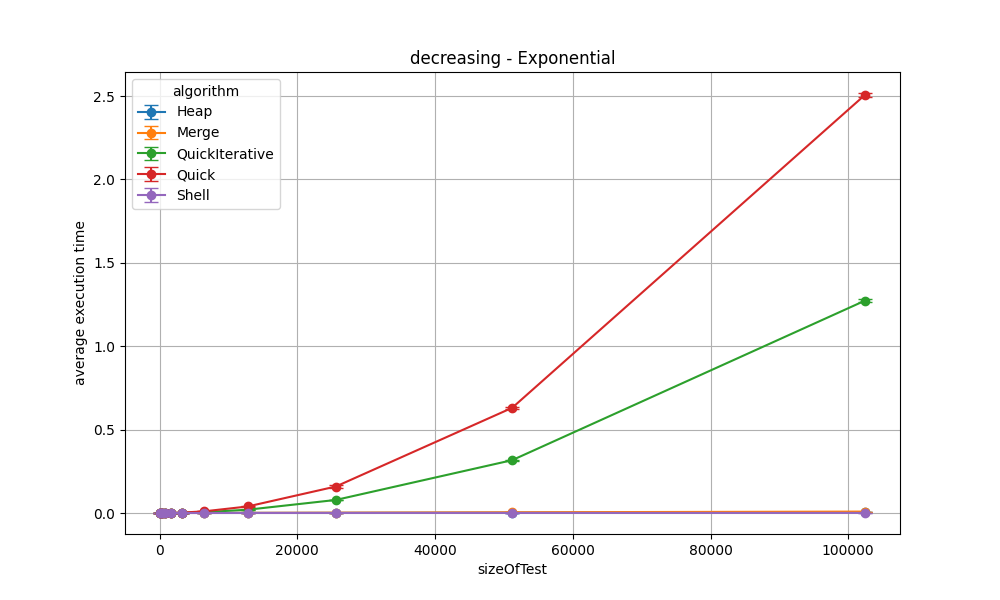
\includegraphics[scale=0.7]{../plotsData/decreasing_Exponential.png}
		\caption{Decreasing – Exponential}
		\label{fig:decreasing_exponential}
	\end{minipage}
	\hfill
	
	\begin{minipage}{0.48\textwidth}
		\hspace*{-5cm}
		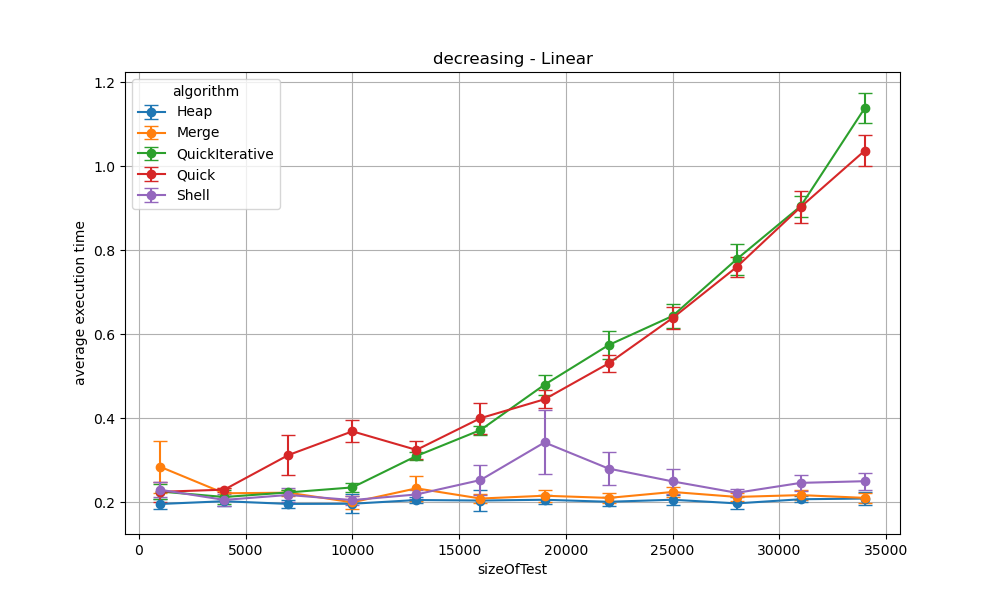
\includegraphics[scale=0.7]{../plotsData/decreasing_Linear.png}
		\caption{Decreasing – Linear}
		\label{fig:decreasing_linear}
	\end{minipage}
	
\end{figure}

\begin{figure}
	\centering
	
	\begin{minipage}{0.48\textwidth}
		\hspace*{-5cm}
		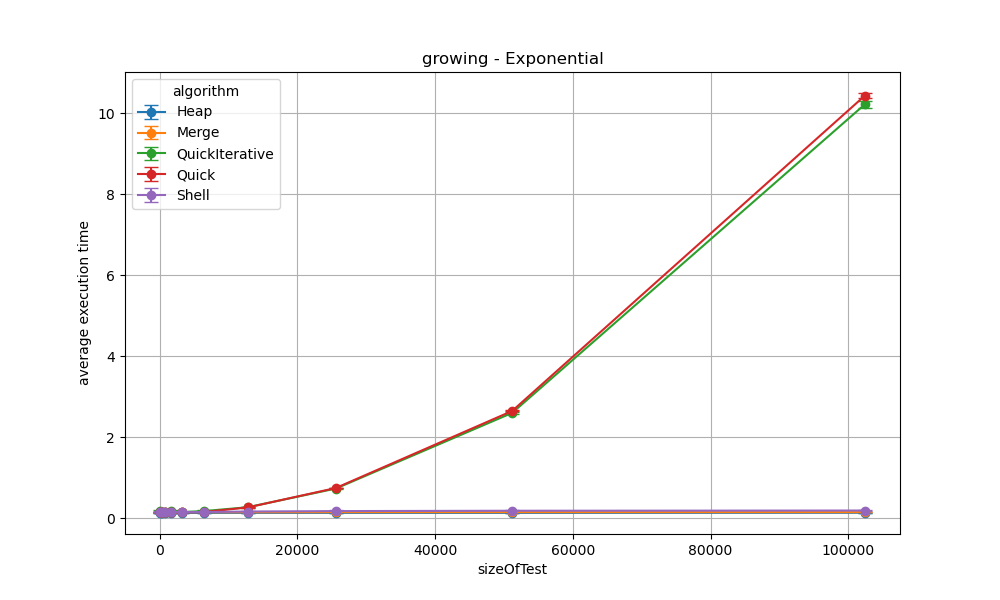
\includegraphics[scale=0.7]{../plotsData/growing_Exponential.png}
		\caption{Growing – Exponential}
		\label{fig:growing_exponential}
	\end{minipage}
	\hfill
	
	\begin{minipage}{0.48\textwidth}
		\hspace*{-5cm}
		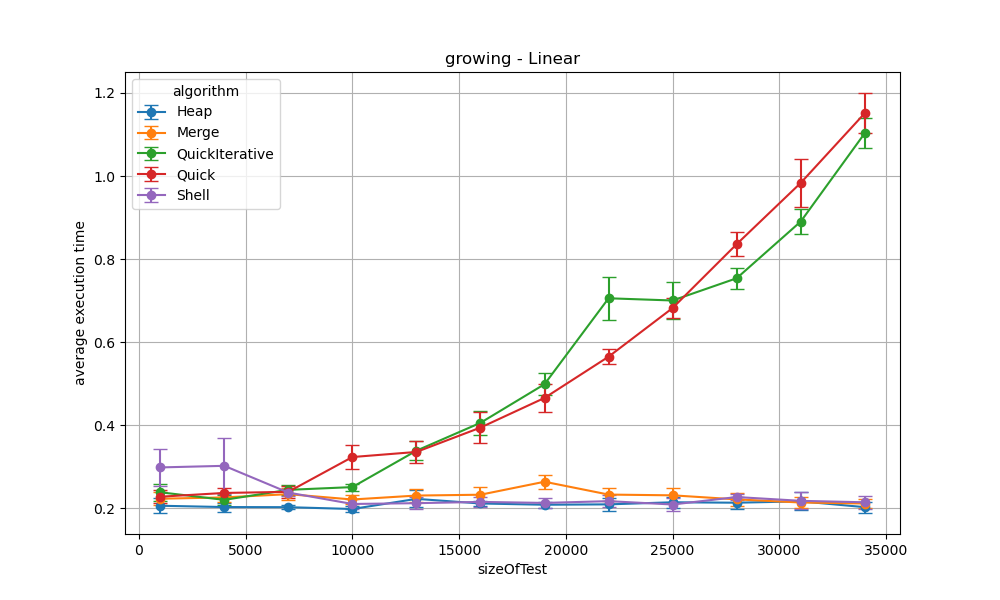
\includegraphics[scale=0.7]{../plotsData/growing_Linear.png}
		\caption{Growing – Linear}
		\label{fig:growing_linear}
	\end{minipage}
	
\end{figure}

\begin{figure}
	\centering
	
	\begin{minipage}{0.48\textwidth}
		\hspace*{-5cm}
		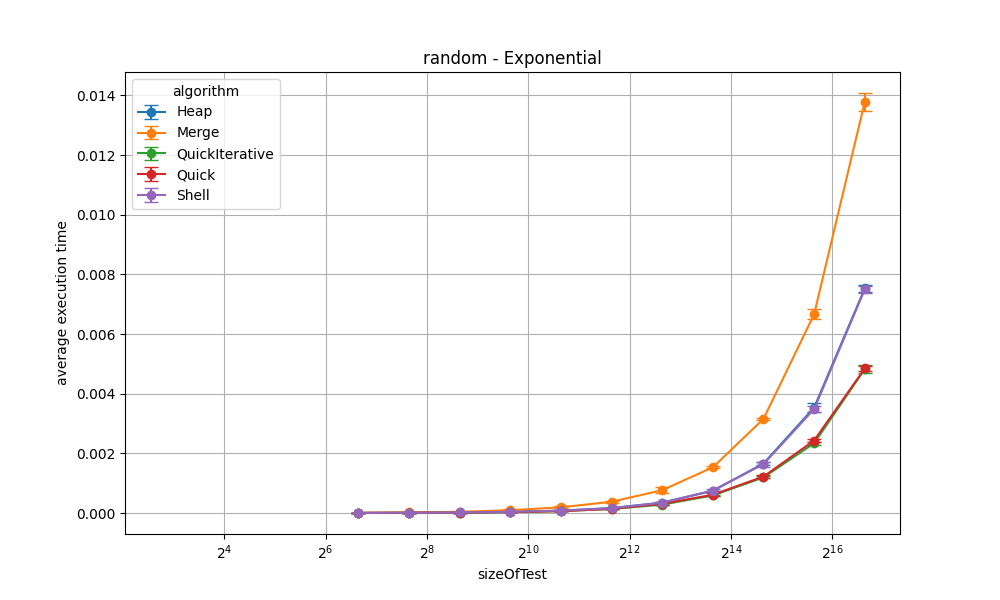
\includegraphics[scale=0.7]{../plotsData/random_Exponential.png}
		\caption{Random – Exponential}
		\label{fig:random_exponential}
	\end{minipage}
	\hfill
	
	\begin{minipage}{0.48\textwidth}
		\hspace*{-5cm}
		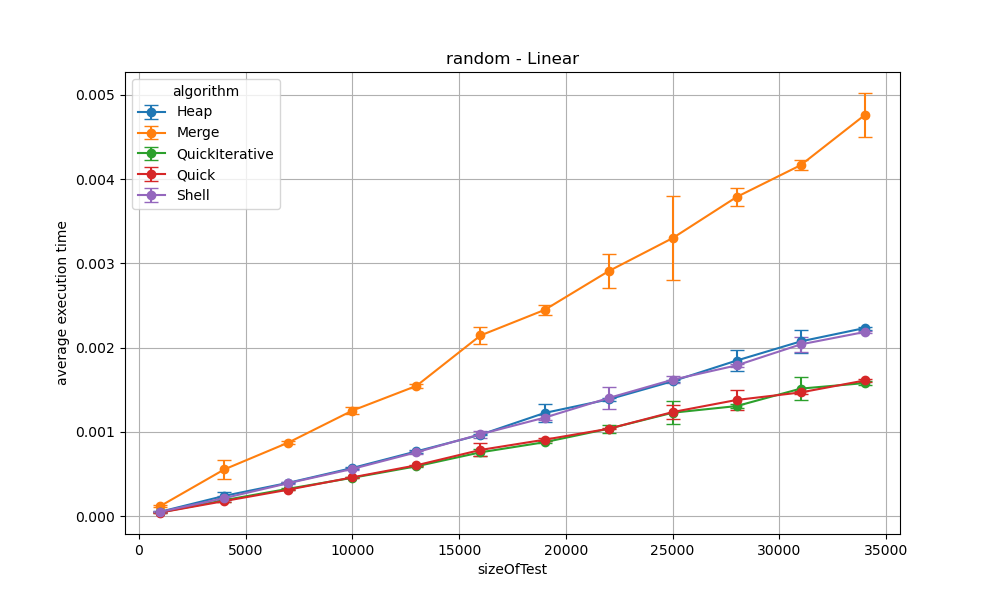
\includegraphics[scale=0.7]{../plotsData/random_Linear.png}
		\caption{Random – Linear}
		\label{fig:random_linear}
	\end{minipage}
	
\end{figure}

\begin{figure}
	\centering
	
	\begin{minipage}{0.48\textwidth}
		\hspace*{-5cm}
		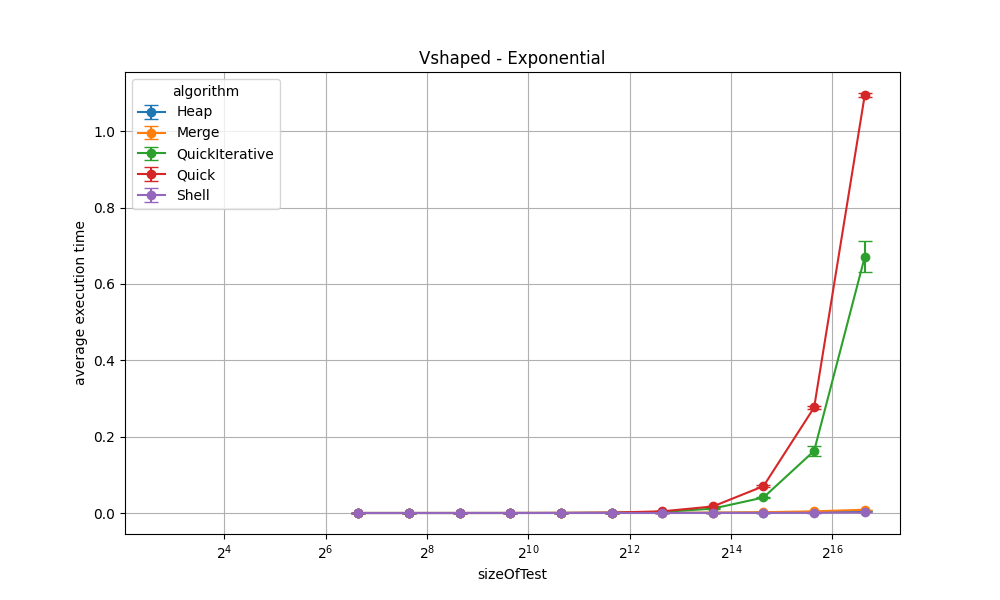
\includegraphics[scale=0.7]{../plotsData/Vshaped_Exponential.png}
		\caption{V-shaped – Exponential}
		\label{fig:vshaped_exponential}
	\end{minipage}
	\hfill
	
	\begin{minipage}{0.48\textwidth}
		\hspace*{-5cm}
		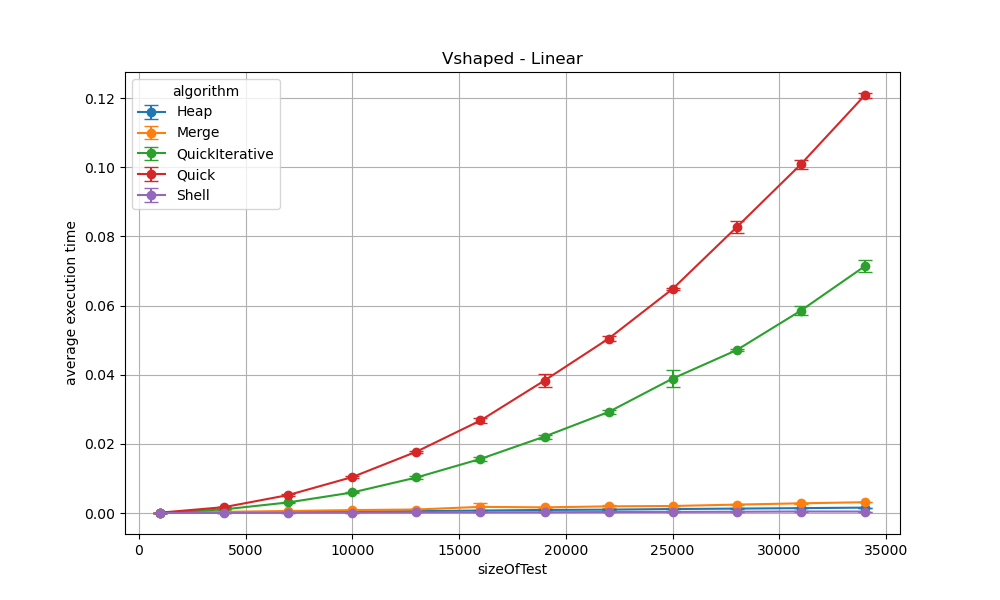
\includegraphics[scale=0.7]{../plotsData/Vshaped_Linear.png}
		\caption{V-shaped – Linear}
		\label{fig:vshaped_linear}
	\end{minipage}
	
\end{figure}
\pagestyle{plain}

\clearpage
\section{Analiza prównawcza eksperymentów.}
\begin{enumerate}
	\item W eksperymencie pierwszym lepiej widać małe różnicę pomiędzy algorytmami. Przez rosnące liniowo długości sortowanych ciągów, można zauważyć różnicę między algorytmami o tych samych złożonościach obliczeniowych.  
	\item Przy wzroście wykładniczym długości sortowanych ciągów krzywe czasu średniego przybierają kształty pokrywające się z teoretyczną złożonością obliczeniową. Linie wykresów nie mają odchyleń od swojego trendu.
	\item Wzrost wykładniczy daje wykresy z mniejszymi odchyleniami od krzywych teoretycznych. dzięki wykładniczo rosnącym długością ciągów pomiary czasu średniego odbywają się dla bardziej różniących się od siebie długości ciągu co pozwala na eliminację zakłóceń lokalnych i  w rezultacie daje wykresy dobrze pokrywające się z teoretyczną złożonością obliczeniową dla danego algorytmu i typu danych.
	\item Dla małych długości ciągów różnicę między czasem pracy poszczególnych algorytmów nie są istotne. W znacznej większości przypadków jakiekolwiek różnicę można zaobserwować dopiero dla ciągów mających powyżej 5000 elementów. Jednym wyjątkiem jest tu Merge sort który źle radzi sobie z ciągami wejściowymi typu losowego, w tym przypadku widzimy różnicę już od początku(to jest dla n<5000).
	\item Odchylenie standardowe ma tendencję rosnącą, którą najlepiej widać dla wykładniczo rosnących n.  Natomiast dla eksperymentu pierwszego nie da się  wskazać ciągłego trendu z uwagi na zakłócenia lokalne, które są widoczne dla mało różniących się od siebie n. Ale eksperyment drugi daje nam obraz mniej podatny na skrajne wartości lokalne i ukazuje stabilny trend rosnący odchylenia standardowego.
	
	
\end{enumerate}

\section{Analiza złożoności obliczeniowej.}
\subsection{Złożoność obliczeniowa dla algorytmów sortowania według rodzaju przypadku:}
$$
\begin{array}{|c|c|c|c|}
	\hline
	\text{Algorytm} & \text{Optymistyczny} & \text{Średni} & \text{Pesymistyczny} \\
	\hline
	\text{Shell Sort} & O(n \log n) & O(n^{3/2}) & O(n^{2}) \\
	\hline
	\text{Merge Sort} & O(n \log n) & O(n \log n) & O(n \log n) \\
	\hline
	\text{Heap Sort} & O(n \log n) & O(n \log n) & O(n \log n) \\
	\hline
	\text{Quick Sort} & O(n \log n) & O(n \log n) & O(n^{2}) \\
	\hline
	\text{Quick Sort Iteracyjny} & O(n \log n) & O(n \log n) & O(n^{2}) \\
	\hline
\end{array}
$$
\subsection{Związek między złożonością teoretyczną, liczbą wykonanych operacji i zaobserwowanym czasem działania:}

Liczba wykonywanych operacji algorytmu rośnie zgodnie z jego złożonością teoretyczną. Czas wykonania jest w przybliżeniu proporcjonalny do liczby tych operacji, jednak zależy również od czynników zewnętrznych, jak na przykład sprzęt lub obciążenie systemu. Dlatego złożoność teoretyczna nie jest obserwowana bezpośrednio, lecz można ją wnioskować z kształtu wzrostu czasu działania dla rosnących rozmiarów danych.

\subsection{Analiza:}
Czy wyniki eksperymentalne potwierdzają analizę teoretyczną?

W jakich przypadkach występują odchylenia oraz z czego mogą wynikać? \\
Przykładem odchylenia jest widoczna na wykresie Heap - Linear nienaturalnie wysoka wartość krzywej random. Najpewniej jest ona spowodowana obciążeniem systemu komputera na którym był przeprowadzany eksperyment.

Z czego mogą wynikać różnice między teorią a pomiarem?

\section{Wnioski końcowe.}
\subsection{Najbardzie efektywny algorytm w praktyce}
\subsection{Algorytm najbardziej wrażliwy na postać danych wejściowych}
\subsection{Porównanie Quick Sort - rekurencyjnego i iteracyjnego}
\subsection{Konsekwencje ustawienia pivot dla Quick Sort}
\subsection{Skalowanie liniowe czy wykładnicze danych wejściowych?}

\end{document}
